\documentclass[UTF8,10pt, twoside]{book}
\usepackage{ctexcap}   %中文支持 
%页面纸张设置
\usepackage{geometry}
\geometry{a4paper, papersize={210mm,297mm}, scale=0.8} %A4
\geometry{left=2cm,right=2cm,top=2cm,bottom=2cm}

% 设置中文段落首行缩进 
\usepackage{indentfirst}
\setlength{\parindent}{2em }  
% 设置行间距
\renewcommand{\baselinestretch }{1.2}
%设置段落间距
\addtolength{\parskip}{.4em}

%章节样式
\usepackage{titlesec}    
\titleformat{\chapter}{\centering\Huge\bfseries}{\chaptername}{1em}{}
\renewcommand{\chaptername}{第~\thechapter~章}
\titleformat{\section}{\LARGE\bfseries}{\thesection}{1em}{}
\titlespacing{\chapter}{0pt}{-20pt}{25pt}


%目录样式  
\CTEXsetup[name={第,章}, number={\arabic{chapter}}]{chapter} 
 

%页眉页脚
\usepackage{fancyhdr}
\pagestyle{fancy}
\fancyhf{}  
\renewcommand{\chaptermark}[1]{\markboth{第\thechapter 章\ ~~#1}{}}
\renewcommand{\sectionmark}[1]{\markright{\thesection ~~#1}{}}
\fancyhead[LO]{\leftmark}    %奇数页左侧章标题
\fancyhead[RE]{\rightmark}  %偶数页右侧节标题
\fancyhead[RO,LE]{-\,\thepage\,-}   %奇数页右侧, 偶数页左侧是页码
\renewcommand{\headrulewidth}{0pt} %无页眉线


%在目录中加入参考文献,索引等,   nottoc 不显示目录本身
\usepackage[nottoc]{tocbibind}

\usepackage{microtype}  %让字体更好看
\usepackage[colorlinks=false, pdfborder={0 0 0}]{hyperref}   %生成引用(图片/表格/公式)超链接

%引入图片,子图宏包
\usepackage{graphicx}
\usepackage{subfigure}
\setcounter{totalnumber}{2} %阻止 Latex将多于两个的浮动对象放置到同一页中
\usepackage{float}   %用于控制浮动
\usepackage[format=hang, font=small, textfont=it]{caption}
\DeclareCaptionLabelSeparator{twospace}{\ ~}
\captionsetup{labelsep=twospace}    %把图注序号与文本之间的冒号分隔符换成两个空格

%直立积分号
\usepackage{amsmath,amssymb}
\DeclareSymbolFont{EulerExtension}{U}{euex}{m}{n}
\DeclareMathSymbol{\euintop}{\mathop} {EulerExtension}{"52}
\DeclareMathSymbol{\euointop}{\mathop} {EulerExtension}{"48}
\let\intop\euintop
\let\ointop\euointop

%脚注样式
\usepackage{pifont}
\usepackage[perpage]{footmisc}  %每页脚注重新编号
\renewcommand{\thefootnote}{\ding{\numexpr191+\value{footnote}}}

%表格样式
\usepackage{multicol} 
\usepackage{multirow}
\usepackage{ctexcap}   
\usepackage{booktabs} 
\usepackage{colortbl}
\definecolor{tabcolor}{rgb}{.105,.410,.113}

%定理样式
\usepackage[T1]{fontenc}
\usepackage[utf8]{inputenc}
\usepackage{amsmath}
\usepackage{boiboites}  
\usepackage{chngcntr}
\newcounter{theoremcounter} 
\counterwithin{theoremcounter}{chapter} 
\newboxedtheorem[
boxcolor=orange,background=blue!5,titlebackground=blue!20,titleboxcolor=black]
{theo}{Theorem}{theoremcounter}


%伪代码/算法
\usepackage[vlined,ruled]{algorithm2e}


%绘图设定
%\usepackage{mathpazo}
\usepackage{tikz} 
\usepackage{pgfplots}
\pgfplotsset{compat=1.8}
\usetikzlibrary{arrows,intersections} 
% TikZ 设定
\tikzset{thick, >=stealth', dot/.style={draw,fill=white,circle,inner sep=0pt,minimum size=4pt}}


%流程图样式 
\usepackage{tikz}
\usetikzlibrary{shapes.geometric, arrows}
 \tikzstyle{startstop} = [rectangle, rounded corners, minimum width=3cm, minimum height=1cm,text centered, draw=black, fill=red!30]
 \tikzstyle{io} = [trapezium, trapezium left angle=70, trapezium right angle=110, minimum width=3cm, minimum height=1cm, text centered, draw=black, fill=blue!30]
 \tikzstyle{process} = [rectangle, minimum width=3cm, minimum height=1cm, text centered, draw=black, fill=orange!30]
 \tikzstyle{decision} = [diamond, minimum width=3cm, minimum height=1cm, text centered, draw=black, fill=green!30]
 \tikzstyle{arrow} = [thick,->,>=stealth]

%强调定义
\newcommand{\Emph}{\textbf}

%取消单词切断
\tolerance=1
\emergencystretch=\maxdimen
\hyphenpenalty=10000
\hbadness=10000


%随机段落,用于示例
\usepackage{lipsum}   
%把指定的章节包含进来,用于分段编译,调试,这里的参数是列表
\includeonly{ch1}

%%%%%%%%%%%%%%%%%%%%%%%%%%%%%%%%%%%%% 
\begin{titlepage}
    \title{\LaTeX{}编辑参考}
    \author{宫庆义\\gongqingyi@qq.com} 
    \date{\today}
\end{titlepage}

%%%%%%%%%%%%%%%%%%%%%%%%%%%%%%%%%%%%%
\begin{document} 
\frontmatter  
\pagestyle{empty}
\maketitle                         %生成标题  
\setcounter{page}{1}        %页码从1开始
\tableofcontents               %生成目录  
\pagestyle{fancy}
%%%%%%%%%%%%%%%%%%%%%%%%%%%%%%%%%%%%%
%\newpage
%\setcounter{page}{1}        %页码从1开始
%\setcounter{chapter}{1}    %章节从1开始
\mainmatter                         %页码,章节都从1开始
%第一章包含进来 
\chapter{导论}
\section{概要}
\lipsum[1]
\subsection{\LaTeX{}的基本命令}

{\kaishu  这里是楷书} \quad {\songti  这里是宋体}
\quad {\heiti  这里是黑体}\quad {\fangsong  这里是仿宋} 

\begin{center}
	 字号示例:\\
	{\zihao{0}初号}
	{\zihao{1}一号}
	{\zihao{2}二号}
	{\zihao{3}三号}
	{\zihao{4}四号}
	{\zihao{5}五号}
	{\zihao{6}六号}
	{\zihao{7}七号}
	{\zihao{8}八号}
\end{center}



北京\footnote{直辖市}是中国的首都\footnote{一个国家的首府}.如图\ref{fig:1}所示
公式\ref{eq:1}是著名的格林公式,公式\ref{eq:2}是复变函数中的柯西公式.
This is \Emph{emphasized} text.\newline
\textit{This is Italic font !}

\begin{multicols}{2}
	\lipsum[1]
\end{multicols}  

\begin{equation}
    \label{eq:1}
	\iint\limits_{{D}} {(\frac{{\partial Q}}{{\partial x}} – \frac{{\partial P}}{{\partial y}})}dxdy = \oint_{L} {Pdx + Qdy}
\end{equation}

\begin{equation}
	\label{eq:2}
	f(z_0)=\frac{1}{2\pi i}\oint_{C}^{ } \frac{f(z)}{z-z_0}dz
\end{equation}
 
 
\begin{figure}[!htbp]   %here or top
	\centering
	\includegraphics[width=5cm]{./image/ch1/0.jpg}
	\caption{this is a pic of $\pi$}
	\label{fig:1}
\end{figure}

\begin{figure}[hbtp]
	\begin{minipage}[t]{0.5\textwidth}
		\centering
		\includegraphics[width=5cm]{./image/ch1/1.jpg}
		\caption{this is a dog}
		\label{fig:side:a}
	\end{minipage}%
	\begin{minipage}[t]{0.5\textwidth}
		\centering
		\includegraphics[width=5cm]{./image/ch1/2.jpg}
		\caption{this is a butterfly}
		\label{fig:side:b}
	\end{minipage}
\end{figure}


\begin{figure}[!hbtp]
	\centering
	\subfigure[this is a  bufferfly ]{
		\label{fig:subfig:a} %% label for first subfigure
		\includegraphics[width=5cm]{./image/ch1/3.jpg} 
	} 
	\hspace{1in}
	\subfigure[this is a beautiful flower]{
		\label{fig:subfig:b} %% label for second subfigure
		\includegraphics[width=5cm]{./image/ch1/4.jpg} 
	}
	\caption{Two Subfigures example}
	\label{fig:subfig} %% label for entire figure
\end{figure}

\begin{multicols}{2}
\lipsum[1]
\end{multicols}  

\begin{theo}
	   [Law of Large Numbers]
		Let $(X_n)_{n\in \mathbb{N}}$ be an infinite sequence of i.i.d. variables with finite expected value. Then:
		$$\frac{1}{n} \sum_{i=1}^n X_i \overset{\textnormal{a.s.}}{\longrightarrow}
		\mathbb{E} (X_1) .$$
\end{theo}

\begin{theo}
	[Law of Large Numbers]
	Let $(X_n)_{n\in \mathbb{N}}$ be an infinite sequence of i.i.d. variables with finite expected value. Then:
	$$\frac{1}{n} \sum_{i=1}^n X_i \overset{\textnormal{a.s.}}{\longrightarrow}
	\mathbb{E} (X_1) .$$
\end{theo}


\begin{multicols}{2}
	\lipsum[1]
\end{multicols}  

\subsection{\LaTeX{}的排版}
\begin{multicols}{2}
	\lipsum[1]
\end{multicols}  

\begin{table}[!htbp]  
	\centering  
	\begin{tabular}{cccccc}  
		\arrayrulecolor{tabcolor} 
		\toprule[1.4pt]   
		     &文科 & 理科 & 工科 & 商科 & 总计 \\  
		\hline  
		男& 77 & 98 & 77 & 98 & 175 \\  
		女& 101 & 72 & 77 & 98 & 173 \\  
		男& 77 & 98 &  77 & 98 &175 \\  
		女& 101 & 72 & 77 & 98 & 173 \\  
		男& 77 & 98 &  77 & 98 &175 \\  
		女& 101 & 72 &  77 & 98 &173 \\  
		总计& 178 & 170 & 178 & 170 &348 \\  
		\bottomrule[1.4pt]  
	\end{tabular}  
	\caption {问卷调查对象基本情况汇总表.}  
	\label{tab:number}  
\end{table}  

 
\SetKwProg{Fn}{Function}{\string:}{}   
\begin{algorithm}[!htbp]  
	\DontPrintSemicolon
	\LinesNumbered
	\caption{IntervalRestriction\label{IR}}
    \Fn{Recurs(X, U)}{
	\KwData{$G=(X,U)$ such that $G^{tc}$ is an order.}
	\KwResult{$G’=(X,V)$ with $V\subseteq U$ such that $G’^{tc}$ is an
		interval order.}
 
		$V \longleftarrow U$\;
		$S \longleftarrow \emptyset$\;
		\For{$x\in X$}{
			$NbSuccInS(x) \longleftarrow 0$\;
			$NbPredInMin(x) \longleftarrow 0$\;
			$NbPredNotInMin(x) \longleftarrow |ImPred(x)|$\;
		}
		\For{$x \in X$}{
			\If{$NbPredInMin(x) = 0$ {\bf and} $NbPredNotInMin(x) = 0$}{
				$AppendToMin(x)$}
		}
	    \While{$S \neq \emptyset$}{\label{InRes1}
		  remove $x$ from the list of $T$ of maximal index\;\label{InResR}
		  \While{$|S \cap ImSucc(x)| \neq |S|$}{
				\For{$ y \in S-ImSucc(x)$}{
					\{ remove from $V$ all the arcs $zy$ : \}\;
					\For{$z \in ImPred(y) \cap Min$}{
						remove the arc $zy$ from $V$\;
						$NbSuccInS(z) \longleftarrow NbSuccInS(z) - 1$\;
						move $z$ in $T$ to the list preceding its present list\;
						\{i.e. If $z \in T[k]$, move $z$ from $T[k]$ to
						$T[k-1]$\}\;
					}
					$NbPredInMin(y) \longleftarrow 0$\;
					$NbPredNotInMin(y) \longleftarrow 0$\;
					$S \longleftarrow S - \{y\}$\;
					$AppendToMin(y)$\;
				}
			}
			$RemoveFromMin(x)$\;
		}
		\Return true
}	 
\end{algorithm}

 
%h浮动体就放在当前页面上。这主要用于小浮动体。
%t 放在页面顶部
%b 放在页面底部
%p 放在一专门页面,仅含一个浮动体。
%!严格按照放置说明符放置即使看起来不好。



\begin{figure}[!hbtp]
\centering
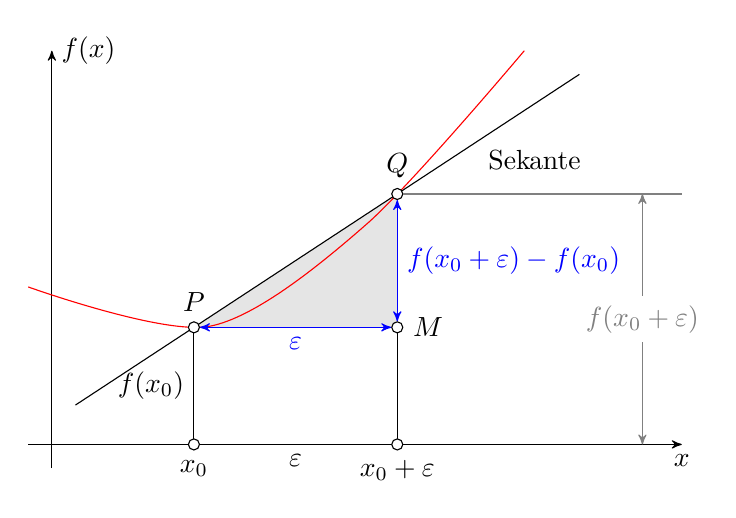
\begin{tikzpicture}
% 画坐标系 并且定义了 O 、xmax 和 ymax
\coordinate (O) at (0,0);
\draw[->] (-0.3,0) -- (8,0) coordinate[label={below:$x$}] (xmax);
\draw[->] (0,-0.3) -- (0,5) coordinate[label={right:$f(x)$}] (ymax);
% 给出直线 x 与曲线 y 的路径
\path[name path=x] (0.3,0.5) -- (6.7,4.7);
\path[name path=y] plot[smooth] coordinates {(-0.3,2) (2,1.5) (4,2.8) (6,5)};

% 利用 intersections 包的计算方法,得到了直线与曲线的交点坐标,分别命名为 i-1 和 i-2 (图中分别为 P 和 Q) 过点 P 的水平线与过 Q 的竖直延长线的交点标记为 M.

\begin{scope}[name intersections = {of= x and y,name = i}]
% 将PQ所形成的三角形区域(PQM)填充为灰色
\fill[gray!20] (i-1) -- (i-2 |- i-1) -- (i-2) -- cycle;
% 在空白处标记 Sekante
\draw (0.3,0.5) -- (6.7,4.7) node[pos=0.8,below right] {Sekante};
% 画出曲线路径 y,与之前代码几乎一样
\draw[red] plot[smooth] coordinates {(-0.3,2) (2,1.5) (4,2.8) (6,5)};
% 从 P 向 x 轴引垂线,垂足坐标为 (i-1 |- O),标签为 x_0
\draw (i-1) node[dot,label={above:$P$}] (i-1) {} -- node[left] {$f(x_0)$} (i-1 |- O) node[dot,label={below:$x_0$}] {};
% Q 点向 M 引垂线
\path (i-2) node[dot,label={above:$Q$}] (i-2) {} -- (i-2 |- i-1) node[dot,label={right:$M$}] (i-12) {};
% M 向 x 轴引垂线,并且标注
\draw (i-12) -- (i-12 |- O) node[dot,label={below:$x_0 + \varepsilon$}] {};
% 连接 Q 与 M,并且标注
\draw[blue,<->] (i-2) -- node[right] {$f(x_0 + \varepsilon) - f(x_0)$} (i-12);
% 连接 P 与 M
\draw[blue,<->] (i-1) -- node[below] {$\varepsilon$} (i-12);
% x 轴上两个垂足之间标记
\path (i-1 |- O) -- node[below] {$\varepsilon$} (i-2 |- O);
% Q 的水平延长线
\draw[gray] (i-2) -- (i-2 -| xmax);
% 标注 Q 点的垂直距离,最精彩的是用到了 xshift=-0.5cm,简直赞!
\draw[gray,<->] ([xshift=-0.5cm]i-2 -| xmax) -- node[fill=white] {$f(x_0 + \varepsilon)$}  ([xshift=-0.5cm]xmax);
\end{scope}

\end{tikzpicture}
\caption{函数的微分}
\label{fig:diff_of_function} %% label for entire figure
\end{figure}



\begin{figure}[!hbtp]
\centering
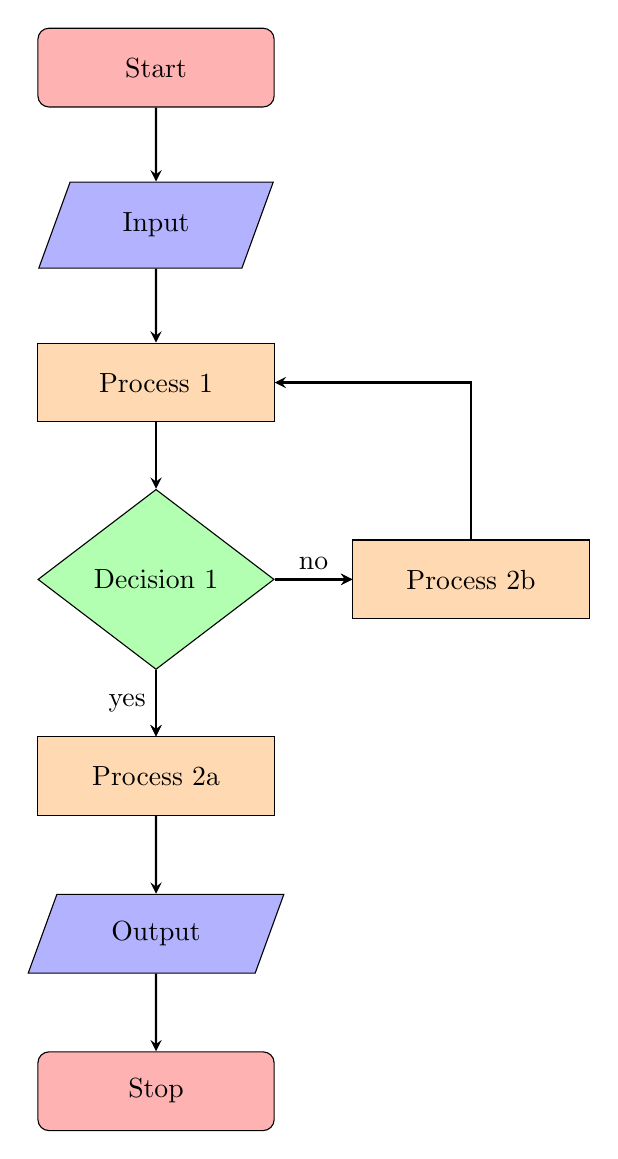
\begin{tikzpicture}[node distance=2cm]
%定义流程图具体形状
\node (start) [startstop] {Start};
\node (in1) [io, below of=start] {Input};
\node (pro1) [process, below of=in1] {Process 1};
\node (dec1) [decision, below of=pro1, yshift=-0.5cm] {Decision 1};
\node (pro2a) [process, below of=dec1, yshift=-0.5cm] {Process 2a};
\node (pro2b) [process, right of=dec1, xshift=2cm] {Process 2b};
\node (out1) [io, below of=pro2a] {Output};
\node (stop) [startstop, below of=out1] {Stop};

%连接具体形状
\draw [arrow](start) -- (in1);
\draw [arrow](in1) -- (pro1);
\draw [arrow](pro1) -- (dec1);
\draw [arrow](dec1) -- (pro2a);
\draw [arrow](dec1) -- (pro2b);
\draw [arrow](dec1) -- node[anchor=east] {yes} (pro2a);
\draw [arrow](dec1) -- node[anchor=south] {no} (pro2b);
\draw [arrow](pro2b) |- (pro1);
\draw [arrow](pro2a) -- (out1);
\draw [arrow](out1) -- (stop);
\end{tikzpicture}
\caption{函数的流程图示例}
\label{fig:flow_of_function} %% label for entire figure
\end{figure}

%函数定义
\tikzset{declare function={ binom(\k,\n,\p)=\n!/(\k!*(\n-\k)!)*\p^\k*(1-\p)^(\n-\k); }}
\begin{figure}[!hbtp]
\centering
\begin{tikzpicture}
\begin{axis}[samples at={0,...,40},
axis lines = left,
xlabel = $x$,
ylabel = {$f(x)$},
yticklabel style={
	/pgf/number format/fixed,
	/pgf/number format/fixed zerofill,
	/pgf/number format/precision=2}
]
\addplot [only marks,orange] {binom(x,40,0.5)};
\addlegendentry{$p=0.5$}
\addplot [only marks,cyan] {binom(x,40,0.2)};
\addlegendentry{$p=0.2$}
\addplot [smooth,thick,orange] {binom(x,40,0.5)};
\addlegendentry{$p=0.5$}
\addplot [smooth,thick,cyan] {binom(x,40,0.2)};
\addlegendentry{$p=0.2$}
\end{axis}
\end{tikzpicture}
\caption{函数的图像}
\label{fig:image_of_function} %% label for entire figure
\end{figure}


\def\layersep{2.5cm}
\begin{figure}[!hbtp]
    \centering
	\begin{tikzpicture}[shorten >=1pt,->,draw=black!50, node distance=\layersep]
	\tikzstyle{every pin edge}=[<-,shorten <=1pt]
	\tikzstyle{neuron}=[circle,fill=black!25,minimum size=17pt,inner sep=0pt]
	\tikzstyle{input neuron}=[neuron, fill=green!50];
	\tikzstyle{output neuron}=[neuron, fill=red!50];
	\tikzstyle{hidden neuron}=[neuron, fill=blue!50];
	\tikzstyle{annot} = [text width=4em, text centered]
	
	% Draw the input layer nodes
	\foreach \name / \y in {1,...,4}
	% This is the same as writing \foreach \name / \y in {1/1,2/2,3/3,4/4}
	\node[input neuron, pin=left:Input \#\y] (I-\name) at (0,-\y) {};
	
	% Draw the hidden layer nodes
	\foreach \name / \y in {1,...,5}
	\path[yshift=0.5cm]
	node[hidden neuron] (H-\name) at (\layersep,-\y cm) {};
	
	% Draw the output layer node
	\node[output neuron,pin={[pin edge={->}]right:Output}, right of=H-3] (O) {};
	
	% Connect every node in the input layer with every node in the
	% hidden layer.
	\foreach \source in {1,...,4}
	\foreach \dest in {1,...,5}
	\path (I-\source) edge (H-\dest);
	
	% Connect every node in the hidden layer with the output layer
	\foreach \source in {1,...,5}
	\path (H-\source) edge (O);
	
	% Annotate the layers
	\node[annot,above of=H-1, node distance=1cm] (hl) {Hidden layer};
	\node[annot,left of=hl] {Input layer};
	\node[annot,right of=hl] {Output layer};
	\end{tikzpicture}
\caption{神经网络结构图}
\label{fig:image_of_neural_net} %% label for entire figure
\end{figure}
 


%以下是附录
\appendix 
\titleformat{\chapter}{\centering\Huge\bfseries}{\chaptername}{1em}{}
\renewcommand{\chaptername}{附录~\thechapter~}
\chapter{数学公式参考}
\chapter{习题答案}

%文献管理工具 JebRef 
%\cite{xxx}  %引用参考文献

\end{document}